\chapter{Классификация существующих решений}

    \section{Существующие решения}
    
    Симметричное шифрование производительнее, чем асимметричное, что делает его более подходящим для отправки данных по HTTPS-соединению. Точный метод генерации ключа зависит от выбранного шифронабора, два самых распространённых из них — RSA и Диффи --- Хеллман.
    

    
   	\subsection{Обмен ключами Diffie --- Hellman, DH}
   	
   	Алгоритм Диффи --- Хеллмана является одним из первых алгоритмов с открытым ключом, предложенным Уитфилдом Диффи (Whitfield Diffie) и Мартином Хеллманом (Martin Hellman) \cite{DH}
   	Данный алгоритм позволил уменьшить требования к каналу связи для установления защищённого соединения без предварительного обмена ключами.
   	
   	
   	Алгоритм позволяет двум сторонам создать общий сеансовый ключ используя такой канал связи, который может прослушивать злоумышленник, но в предположении, что последний не может менять содержимое сообщений.
   	
   	\textbf{Ключ}
   	
   	Для того чтобы установить ключ, клиенту и серверу необходимо выполнить следующие действия.
   	
   	\begin{enumerate}
   		\item Клиент генерирует число \(a\), вычисляет число
   		\begin{equation}
   			A = g^a \bmod p 
   			\label{eq1:ref}
   		\end{equation} 
   		и посылает его серверу.
   		\item Сервер генерирует число \(b\), вычисляет число 
   		\begin{equation}
   			B = g^b \bmod p 
   			\label{eq2:ref}
   		\end{equation}
   		и посылает его клиенту.
   		\item Клиент вычисляет значение
   		\begin{equation}
   			B^a \bmod p = g^{ab} \bmod p 
   			\label{eq3:ref}
   		\end{equation}.
   		\item Сервер вычисляет значение
   		\begin{equation}
   			A^b \bmod p = g^{ab} \bmod p 
   			\label{eq4:ref}
   		\end{equation}.
   	\end{enumerate}
   
   	
   Заметим что обе стороны вычисляют одно и тоже значение

	\begin{equation}
		K = g^{ab} \bmod p.
		\label{eq5:ref}
	\end{equation}

	Таким образом, числа \(p\) и \(q\) можно разослать всем участникам системы.
	
	\begin{figure}[h!]
		\centering
		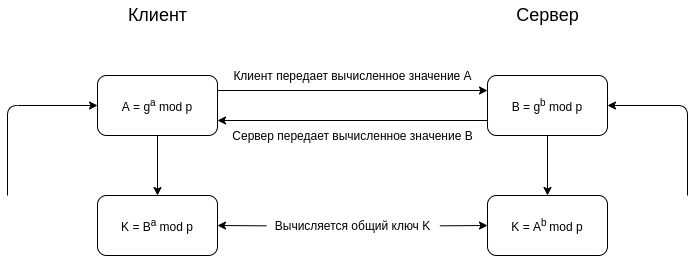
\includegraphics[width=\textwidth,height=7cm,keepaspectratio]{DH.png}
		\caption{Алгоритм шифрования сеансового ключа.} \label{fig:hd}
	\end{figure}
   
   	\subsection{Обмен ключами RSA}
   	
   	
   	Алгоритм RSA носит имя в честь своих создателей Рона Ривест (Ron Rivest), Ади Шамира (Adi Shamir) и Леонарда Адлемана (Leonard Adleman) из Массачусетского технологического института. 
   	
   	Называть это обменом ключами RSA на самом деле неправильно. На самом деле это RSA-шифрование. RSA использует асимметричное шифрование для создания ключа сеанса. 
   	
   	%h \cite{RSA}
   	
   	\textbf{Ключ}
   	
   	Для того чтобы установить ключ, клиенту необходимо выполнить следующие действия.
   	
   	\begin{enumerate}
   		\item Выбрать два различных случайных простых числа \(p\) и \(q\), удовлетворяющих условию \(\mid p \mid \approx\ \mid g\mid \).
   		\item Вычислить \(N = pq\).
   		\item Вычислить 
   		\begin{equation}
   			\phi (N) = (p - 1)(q - 1).
   			\label{eq2.1:ref}
   		\end{equation}
   		\item Выбрать случайное целое число \(e < \phi(N)\) и найти целое число \(d\) такое что
   		\begin{equation}
   			de \equiv  1\bmod\phi(N).
   			\label{eq2.2:ref}
   		\end{equation}
   		\item Использовать пару \((N, e)\) в качестве параметров открытого ключа, тщательно уничтожить числа \(p, g, \phi(N)\) и запомнить число \(d\) в качестве закрытого
   		ключа.
   	\end{enumerate}
   	
   	\textbf{Шифрование}
   	
   	Для того чтобы переслать клиенту секретное сообщение, имеющее длину \(m < N\) ,
   	сервер создает зашифрованный текст 
   	\[c = m^e\pmod N\]
   	
   	\textbf{Расшифровка}
   	
   	Для того чтобы расшифровать зашифрованный текст \(c\), клиент вычисляет формулу \[m = c^d\pmod N\]
   	
   	\begin{figure}[h!]
   		\centering
   		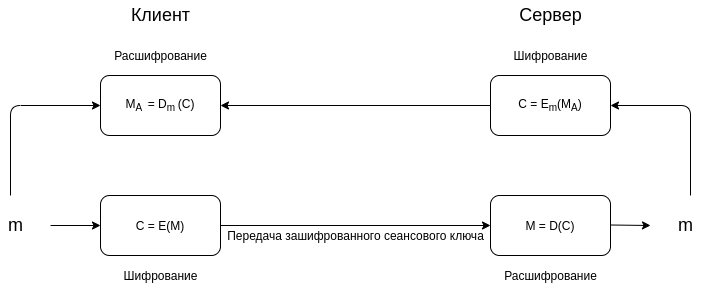
\includegraphics[width=\textwidth,height=7cm,keepaspectratio]{rsa.png}
   		\caption{Алгоритм шифрования сеансового ключа.} \label{fig:rsa}
   	\end{figure}
   
   

   	\newpage
   	
   	\section{Критерий по колличеству ключей}
   	
   	\textbf{Симметричное шифрование} --- это метод использования одних и тех же криптографических ключей как для шифрования открытого текста, так и для дешифрования зашифрованного текста.
   	
   	\textbf{Асимметричное шифрование} --- это метод использования пары ключей: открытого ключа, который широко распространен, и частного ключа, который известен только владельцу.
   	
   	 \begin{figure}[h!]
   		\centering
   		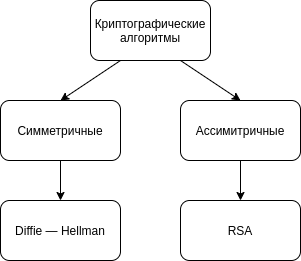
\includegraphics[width=\textwidth,height=8cm,keepaspectratio]{keys.png}
   		\caption{Критерий по колличеству ключей} \label{fig:keys}
   	\end{figure}
        
    \section{Активные атаки на криптосистемы}
    
    \subsection{Атака "человек посередине" (man-in-the-middle attack --- MITM)}
    
    Вид атаки, когда злоумышленник тайно ретранслирует и при необходимости изменяет связь между двумя сторонами, которые считают, что они непосредственно общаются друг с другом.
    
    \subsection{Атака на основе подобранного открытого текста (chosen-plaintext attack ---
    CPA).} 
	Атакующий выбирает исходные сообщения и передает их шифровальщику для получения зашифрованных текстов. Задача атакующего — взломать криптосистему, используя полученные пары открытых и зашифрованных текстов.
    
    \subsection{Атака на основе подобранного зашифрованного текста (chosen-ciphertext attack --- CCA).} 
	Атакующий выбирает зашифрованные сообщения и передает их на расшифровку для получения исходных сообщений. Цель атакующего — взломать криптосистему, используя полученные пары открытых
    и зашифрованных текстов. Атакующий достигает успеха, если он раскрывает ключ и способен в дальнейшем извлекать секретную информацию из
    зашифрованного текста, не прибегая к посторонней помощи.
    
    \subsection{Атака на основе адаптивно подобранного зашифрованного текста (adaptive chosen-ciphertext attack --- CCA2).} 
	Это — разновидностьатаки CCA, в которой услуги расшифровки доступны для всех зашифрованных текстов, за
    исключением заданного.
 
 	
 	
	 \begin{table}[h!]
		\begin{center}
			\caption{Классификация по атакам на криптосистемы.}
			\label{tbl:attack}
			\begin{tabular}{|p{2.5cm}|p{5cm}|p{5cm}|}
				\hline \textbf{} & \textbf{Diffie --- Hellman} & \textbf{RSA}  \\
				\hline \textbf{MITM} & \textbf{+} & \textbf{-} \\
				\hline \textbf{CPA} & \textbf{} & \textbf{} \\
				\hline \textbf{CCA} & \textbf{} & \textbf{}  \\
				\hline \textbf{CCA2} & \textbf{} & \textbf{} \\
				\hline
			\end{tabular}
		\end{center} 		
		
	\end{table}
        
    

    \section{Вывод}
    
    RSA облегчает обмен ключами, позволяя клиенту шифровать общий секрет и отправлять его на сервер, где он используется для вычисления соответствующего сеансового ключа. Обмен ключами DH на самом деле вообще не требует обмена открытым ключом, скорее обе стороны создают ключ вместе.

        